\documentclass[border=2pt]{standalone}
\usepackage{tikz}
\usetikzlibrary{decorations.text}
\begin{document}
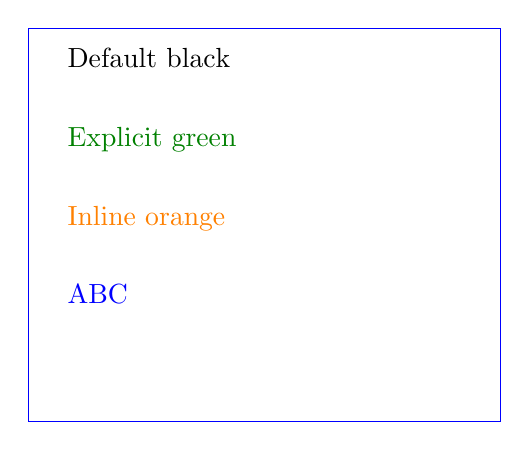
\begin{tikzpicture}
  \draw[blue] (-.5,-.5) rectangle (5.5,4.5);
  \draw[red,text=blue,decorate,decoration={text along path,text={Default black}}] (0,4) -- (5,4);
  \draw[red,decorate,decoration={text along path,text color=green!50!black,text={Explicit green}}] (0,3) -- (5,3);
  \draw[red,decorate,decoration={text along path,text color=green,text={|\color{orange}|Inline orange}}] (0,2) -- (5,2);
  \draw[red,text=blue,decorate,decoration={text effects along path,text={ABC},
    text effects/.cd,characters={text along path}}] (0,1) -- (5,1);
\end{tikzpicture}
\end{document}
